\documentclass[journal,12pt,twocolumn]{IEEEtran}
\usepackage[utf8]{inputenc}
\usepackage{graphicx}
\usepackage{amssymb}
\usepackage{amsmath}
\title{Assignment 1}
\author{Kotikalapudi Karthik \\
CS21BTECH11030}
\date{29th March 2022}

\begin{document}

\maketitle

\section*{ICSE 2018 Question 9 (c)}
\begin{figure}[ht!]
	  \centering 
	  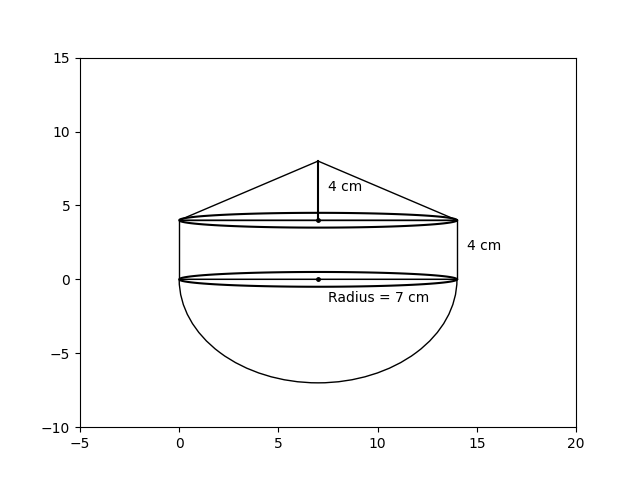
\includegraphics[width=\columnwidth]{Figs/question9c.png}
\end{figure}
\textbf{Solution :}\\
Here,\\
Radius of cone = Radius of cylinder = Radius of hemisphere = $7cm$\\
Height of cone = Height of cylinder = $4cm$\\
Volume of the figure = Volume of cone + Volume of cylinder + Volume of hemisphere
\begin{align}
    \text{Volume of cone} &= \frac{1}{3} \pi r^2 h
    \\
    \text{Volume of cylinder} &= \pi r^2 h
    \\
    \text{Volume of hemisphere} &= \frac{2}{3} \pi r^3
\end{align}
$\therefore$From the above equations,\\
Volume of the figure = $\frac{1}{3} \pi r^2 h + \pi r^2 h + \frac{2}{3} \pi r^3$\\
$\implies$ Volume of the figure
\begin{align*}
    &= \frac{2}{3} \pi r^2 (2h+r)\\
    \text{By substituting $h$ and $r$,}\\
    \text{Volume of the figure}\\
    &= \frac{2}{3} 49 (8+7) \pi\\
    &= 490 \pi\\ 
    &\approx 1539.38cm^3
\end{align*}
\end{document}
